% Appendix A

\chapter{TopFCNH} % Main appendix title

\label{AppendixB} % For referencing this appendix elsewhere, use \ref{AppendixA}

% outline
%----------------------------------------------------------------------------
% 
%
\section{Introduction}

Besides my work on the Fast Calorimeter Simulation Challenge, I have also been involved in the TopFCNH project. For the sake of better understanding the concept and workflow of an analysis. This project aims to study the the interaction between top quark, higgs boson, and a light quark (u or c) in the context of the Standard Model Effective Field Theory (SMEFT) and search for new physics phenomena. It's just at the beginning stage, so what I have done includes roundtable presentation, gridpack preparation, monte carlo and data comparison. In this appendix, I will provide an overview of the TopFCNC project, the analysis workflow, gridpack generation, and the current status of the project.

\section{Background}

While higgs boson has been discovered in 2012, which is the newest particle, and the LHC is mainly designed for observing it, the top quark is the heaviest known elementary particle in the Standard Model (SM). The interaction between top quark and higgs boson is of great interest, as it can provide many insights into many unknown field.

The top-quark flavor-changing neutral current (TopFCNC) decay $t \to Hq$ (where $q = u, c$) is highly suppressed in the Standard Model (SM) due to the Glashow-Iliopoulos-Maiani (GIM) mechanism. \cite{maiani_gim_2013} The predicted SM branching ratio for this process is $BR(t \to Hq) \sim 10^{-15} - 10^{-13}$, making it practically unobservable at the LHC. However, many beyond-the-SM (BSM) theories predict significantly enhanced branching ratios, making it a promising channel for new physics searches. As you can see the figure \ref{fig:TopFCNC}

\begin{figure}[htbp]
    \centering
    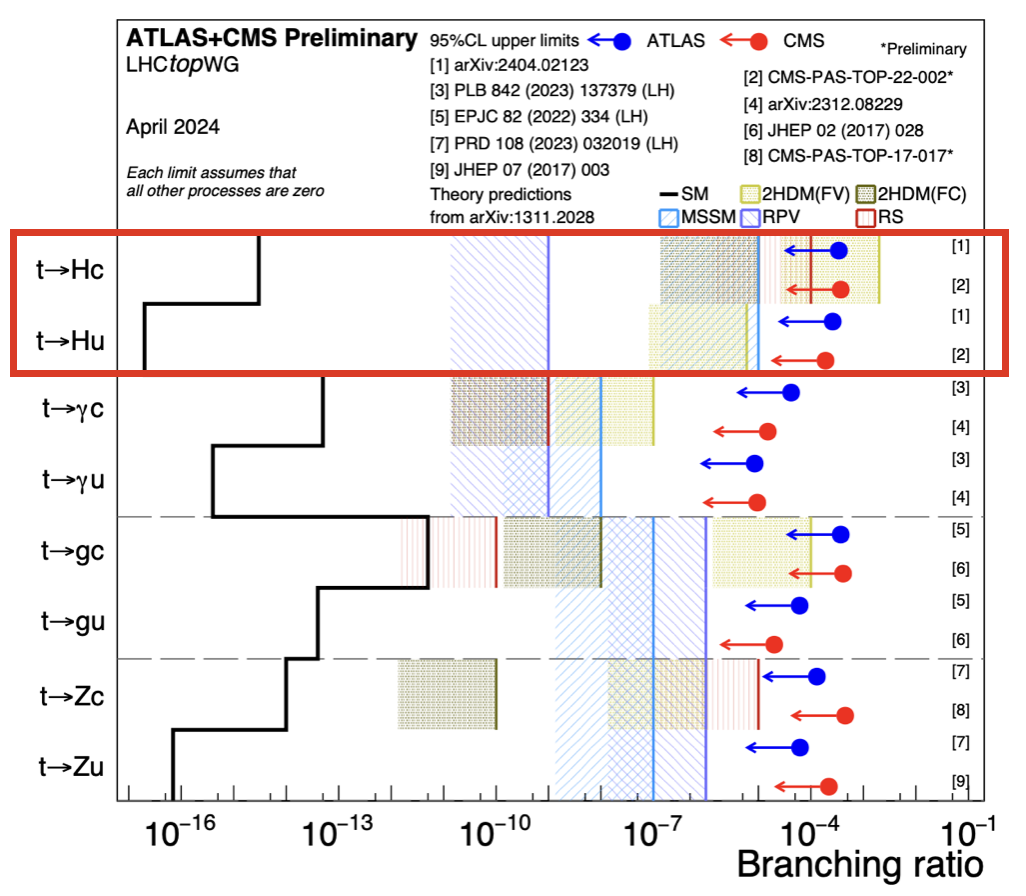
\includegraphics[width=0.8\textwidth]{Figures/topfcnc.png}
    \caption{The prediction and the result so far}
    \label{fig:TopFCNC}
\end{figure}

Several BSM frameworks predict an increase in the branching ratio. The Two-Higgs Doublet Model (2HDM) suggests that $BR(t \to Hq)$ could reach $10^{-5} - 10^{-3}$.\cite{noauthor_fcnchistory_nodate} Similarly, Supersymmetric Models (SUSY) predict comparable enhancements. Additionally, theories involving a Composite Higgs and Extra Dimensions indicate the possibility of increasing the branching ratio to $10^{-4} - 10^{-3}$. Given these enhancements, detecting $t \to Hq$ at the LHC would be a clear sign of new physics.

Among the Higgs boson decay channels, the $H \to \gamma\gamma$ (diphoton decay) is particularly attractive due to its clean experimental signature in the CMS electromagnetic calorimeter. The branching ratio of $H \to \gamma\gamma$ for a 125 GeV Higgs is approximately $0.2\%$, which is small but provides a well-reconstructed final state. Our research focuses on the process $pp \to t\bar{t}$ , $pp \to tH$ and $pp \to tW-$, with $H \to \gamma\gamma$, where the diphoton final state can be efficiently detected using high-resolution electromagnetic calorimetry. The demonstrated Feymann diagram is shown in Figure \ref{fig:TopFCNC_channels}.

\begin{figure}[htbp]
    \centering
    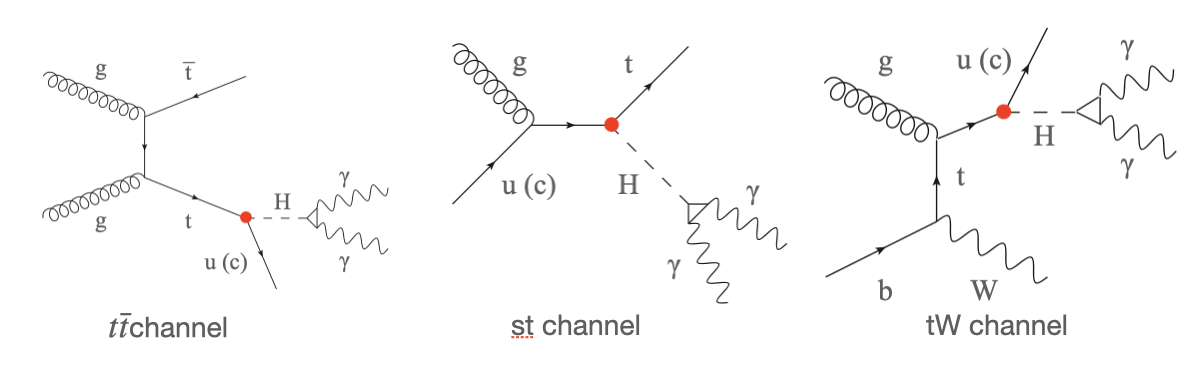
\includegraphics[width=0.8\textwidth]{Figures/topfcnc_channels.png}
    \caption{The Feynman diagrams for the TopFCNC channels}
    \label{fig:TopFCNC_channels}
\end{figure}

Photon triggers in CMS have high efficiency, with single-photon triggers reaching efficiencies above $99\%$ and double-photon triggers capturing over $88\%$ of events. Major backgrounds include prompt diphoton production ($pp \to \gamma\gamma + \text{jets}$) and fake $\gamma + j $, which can be reduced by later analysis methods.

\section{Analysis Tool}

Before we dive into the details of the analysis, let's first introduce the tool, HiggsDNA, we use for the analysis. HiggsDNA stands for Higgs diphoton NANOAOD, which is a tool for analyzing the Higgs boson decay to diphoton in the NanoAOD format. It is a pure Python package, which means the user can do things without CMS environment, that provides a set of functions to analyze the Higgs boson decay to diphoton. 

Besides the environment independence, HiggsDNA also has some other changes and advantages compared to the traditional analysis tool.

First,traditional high-energy physics analyses often employ a per-event processing method, iterating through each event and its components sequentially. While straightforward, this approach can be computationally intensive and time-consuming. HiggsDNA adopts a columnar analysis paradigm, utilizing libraries such as awkward-array and coffea. This method processes data in a vectorized manner, enabling simultaneous operations on entire datasets. Such an approach not only accelerates computations but also enhances code clarity and maintainability.

Second, it provides robust tools to define and propagate these uncertainties throughout the analysis workflow, ensuring that results reflect both statistical and systematic variations.

Third, it also provides the studied corrections for each year, which can be used to correct the data and simulation.

In practice, we incorporate all these pre-studied corrections and uncertainties into a file called \textit{run\_analysis.py}, which calls a processor to handle the data, apply the necessary corrections, and propagate uncertainties to both the data and the simulation. In this process, our main tasks are to write the processor and the analysis code. Once these are prepared, we simply run \textit{run\_analysis.py} to obtain the results.

The overall workflow of the analysis is shown in Figure~\ref{fig:higgs}.

\begin{figure}[htbp]
    \centering
    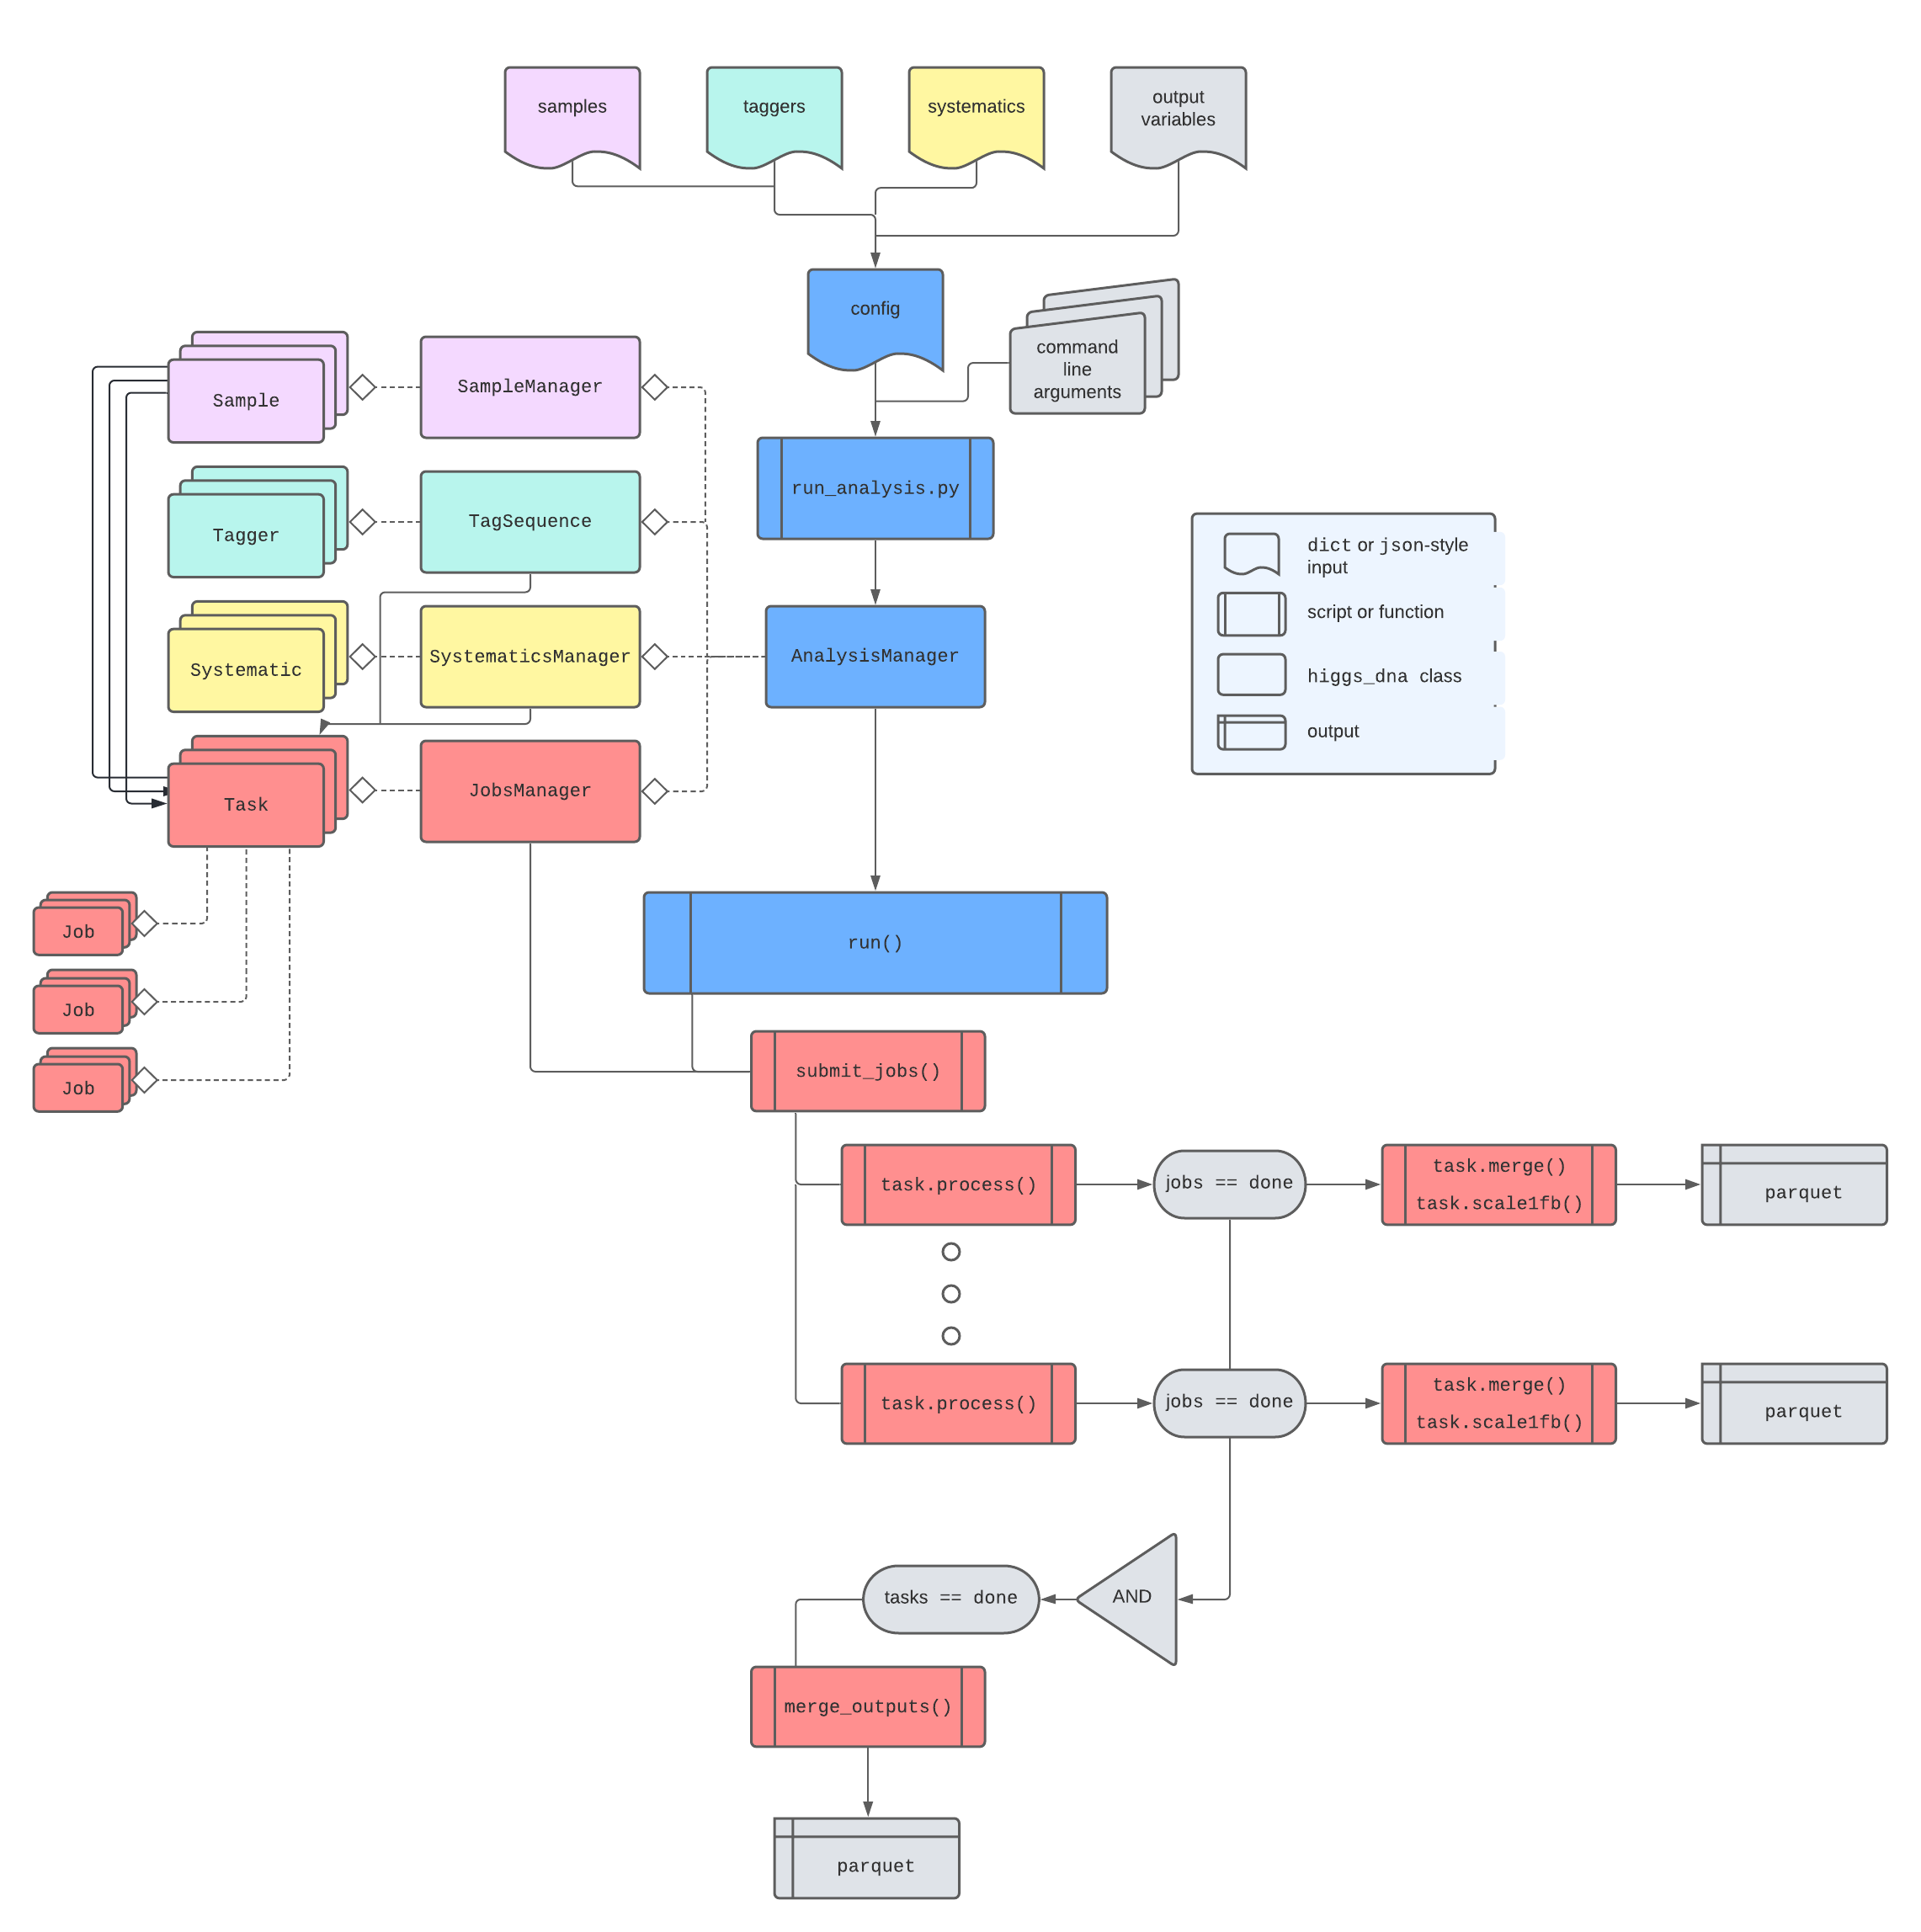
\includegraphics[width=0.8\textwidth]{Figures/higgs_dna.png}
    \caption{The workflow of HiggsDNA.}
    \label{fig:higgs} \cite{higgs_dna}
\end{figure}

 % Move citation outside caption

\section{Workflow}

Although the TopFCNC analysis is still in its early stages, we have established a preliminary workflow to guide our research. The workflow consists of several key steps, each contributing to the overall analysis process. The overall workflow consists of three main stages: Data-MC Samples Comparison \& Top Reconstruction, Signal-Background Separation \& Signal Region Optimization, and Statistical Analysis. This section outlines the key steps in each stage and their significance in the overall analysis.

\subsection{Data-MC Samples Comparison \& Top Reconstruction}
The first step in the analysis workflow involves comparing data and Monte Carlo (MC) samples to validate the simulation's accuracy in modeling real experimental conditions. This stage focuses on reconstructing the top quark and verifying its properties against theoretical predictions. The main aspects of this step include:

\begin{itemize}
\item Utilizing Run 3 data collected between 2022 and 2024.
\item Studying a total of 12 analysis channels, derived from three different production mechanisms and two possible decay modes:
\begin{itemize}
\item Flavored Higgs couplings: Hut and Hct.
\item W boson decays into either leptonic or hadronic final states.
\item Single-top production (st), top-pair production ($t\bar{t}$), and associated top-W production (tW).
\end{itemize}
\item Performing event reconstruction using:
\begin{itemize}
\item A $\chi^2$ method for selecting the most probable event topology.
\item Artificial Neural Network (ANN) training to improve event classification.
\end{itemize}
\end{itemize}

This stage ensures that the data used in the analysis is well understood and that the top quark events are reconstructed with high precision.

\subsection{Signal-Background Separation \& Signal Region Optimization}
Once events are reconstructed, the next stage involves distinguishing signal events from background contributions. This process is critical for maximizing the sensitivity of the analysis. The main components of this stage are:

\begin{itemize}
\item \textbf{Signal-Background Separation:}
\begin{itemize}
\item Multi-Variate Analysis (MVA) techniques are employed, incorporating kinematic features and top reconstruction information.
\item Dedicated MVA classifiers are trained to differentiate between the Higgs signal and backgrounds, including Non-Resonant Background (NRB) and Standard Model Higgs Background (SMH).
\end{itemize}
\item \textbf{Signal Region Optimization:}
\begin{itemize}
\item Signal regions are defined using a two-dimensional phase space, where classification scores from NRB-MVA and SMH-MVA are used to optimize the separation of signal and background events.
\end{itemize}
\end{itemize}

These steps ensure that the analysis isolates the signal efficiently while minimizing background contamination, thereby improving the precision of the final measurement.

\subsection{Statistical Analysis}
The final stage of the workflow involves statistical modeling and interpretation of the extracted signal. This stage includes:

\begin{itemize}
\item \textbf{Modeling:}
\begin{itemize}
\item The invariant mass of the diphoton system ($m_{\gamma\gamma}$) is used as the key observable.
\item Background modeling is performed separately for NRB and SMH components.
\item The sideband regions are defined within the ranges $[100,115] \cup [135,180]$ GeV.
\item The signal window is restricted to $[115,135]$ GeV.
\end{itemize}
\item \textbf{Results:}
\begin{itemize}
\item A simultaneous signal-plus-background (S+B) fit is performed to extract the Higgs boson signal strength.
\item The final step involves setting an upper limit on the branching ratio (BR) of the targeted decay mode.
\end{itemize}
\end{itemize}

This stage quantifies the statistical significance of the observed signal and provides constraints on Higgs boson properties based on the analyzed dataset.

\subsection{Summary of the Workflow}
The entire analysis workflow is summarized in Figure \ref{fig:workflow}. It illustrates the three major stages, from data preparation to final statistical inference. Each step is designed to systematically refine the dataset, enhance the signal-to-background ratio, and extract meaningful physics results from the experimental data.

\begin{figure}[htbp]
\centering
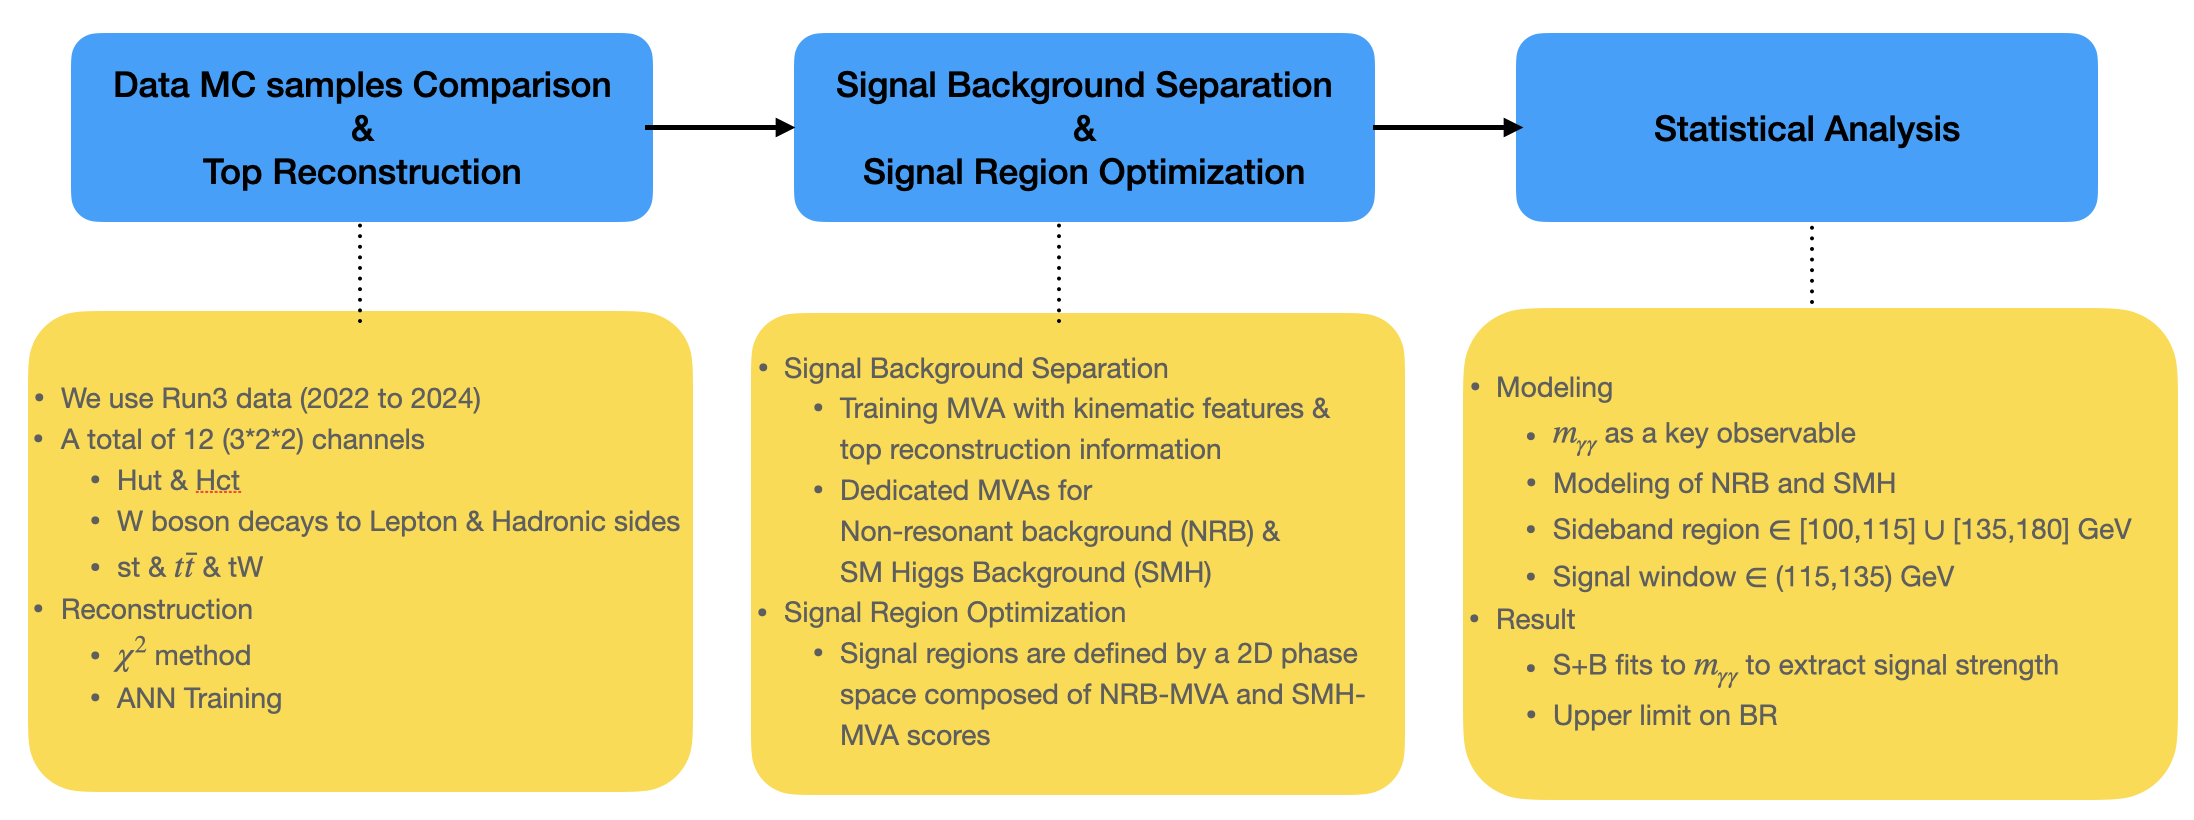
\includegraphics[width=0.9\textwidth]{Figures/workflow.png}
\caption{The workflow of the HiggsDNA analysis framework.}
\label{fig:workflow}
\end{figure}

This structured approach ensures a robust and efficient methodology for Higgs boson studies, leveraging advanced data analysis techniques and statistical tools.

\section{Gridpack Generation}

Originally, this shouldn't be a big problem. However, we faced some difficulties which will be explained later during doing the NLO calculation. In order to generate the signal samples for the TopFCNH ananlysis, we need to create gridpacks which contains all the parameters and configurations for the simulation. The gridpack generation process involves several key steps:

\begin{itemize}
\item \textbf{MadGraph5 Generation} 
The first step is to do the first decay, there are three channels in our research. The first channel is $pp \to t\bar{t}$, the second channel is $pp \to tH$, and the third channel is $pp \to tW-$. It is here that we do the NLO calculation. And the t and W will be decayed in madspin again. 
\item \textbf{Madspin Decay:} 
In this step, we will futher decay $t \to qH$ or $t \to bW+$ and $W \to j j$ or $W \to l \nu$, where $q = u, c$ and $l = e, \mu$.
\item \textbf{Pythia8 Showering:}
The final step is to do the showering and hadronization using Pythia8.
\end{itemize}

However, due to the forbidden process $t \to qH$ in SM, we need to use special model with special parameters designed for TopFCNH. This is the main difficulty we faced during the gridpack generation.
The original model in CMS failed to do the NLO calculation due to the improper parameter settings and python version inconsistency. We need to modify the model and the parameters to make it work. At the end, we also discussed with ATLAS modeling group to get the workable model and parameters. Thus, I also made a presentaion in formal meeting to introduce the work we have done and the problems we faced.

\section{Current Status}

The TopFCNH analysis is still in its early stages, with the gridpack generation being the primary focus. Besides the gridpack generation, we have also started to do the top reconstruction and compare the data and MC samples. For top reconstruction, because we don't have the signal samples yet, we used the ttbar samples to do the reconstruction also for the sake of practicing the HiggsDNA tool.  The results are shown in Figure \ref{fig:TopFCNC_reconstruction}.

\begin{figure}[htbp]
    \centering
    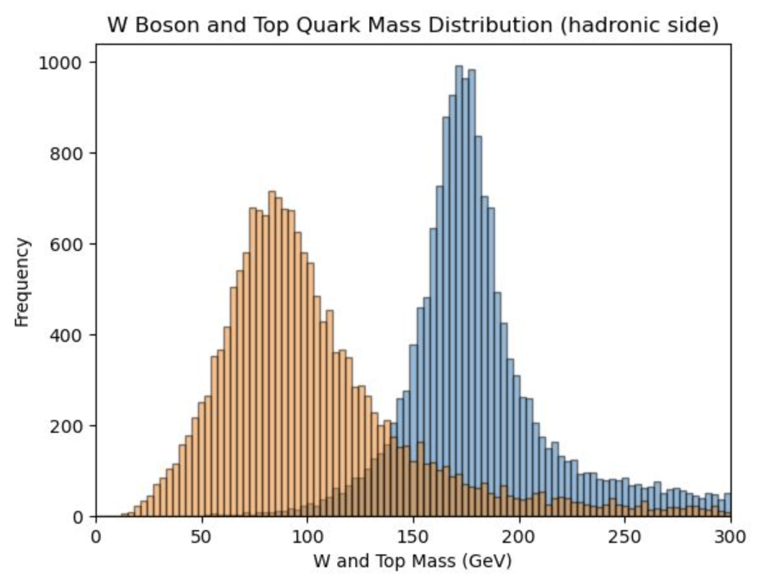
\includegraphics[width=0.8\textwidth]{Figures/TopFCNC_reconstruction.png}
    \caption{Top quark reconstruction using Higgs DNA package (with ttH samples as practice)}
    \label{fig:TopFCNC_reconstruction}
\end{figure}